\documentclass[conference]{IEEEtran}
\IEEEoverridecommandlockouts

\usepackage{amsmath,amssymb,amsfonts}
\usepackage{comment}
\usepackage{graphicx}
\usepackage{textcomp}
\usepackage{xcolor}
\usepackage{biblatex}
\usepackage{float}
\usepackage{caption} 
\usepackage{subcaption}
\usepackage[utf8]{inputenc}
\usepackage[english]{babel}
\usepackage[utf8]{inputenc}
\usepackage{fancyhdr}
\usepackage{biblatex}
\usepackage{hyperref}
\usepackage{algorithm}
\usepackage{algpseudocode}


\addbibresource{sources.bib}

\title{Data partitioning techniques in distributed data intensive systems}
\author{
  Grosu, Cristian (0721808)
  \and
  Teeuwissen, Jelle (6456944)
}
\date{June 2022}

\begin{document}

\maketitle

\pagestyle{fancy}
\fancyhf{}
\rhead{Data Intensive Systems}
\rfoot{Page \thepage}


\section{Introduction}
\label{Section:Introduction}
In the era of digitisation, information became the new gold. The amount of data produced increases each day, especially due to the internet where users themselves produce more data and automated machine systems produce a considerable amount of data (e.g. sensor readings). The need to store and analyse this large amount of data resulted in the apparition of big data, which is characterised by four V's: Volume, Variety, Velocity and Veracity.
Systems like HDFS attempt to tackle the efficient storing and retrieval of the data in a distributed manner. While frameworks like \href{https://hadoop.apache.org/docs/stable/hadoop-mapreduce-client/hadoop-mapreduce-client-core/MapReduceTutorial.html}{Hadoop MapReduce} and \href{https://spark.apache.org/}{SPARK} are used to efficiently query this information to acquire insight. In this paper, we will consider algorithms that run on top of SPARK to cluster data from a structured table consisting of records (i.e. tuples).

\paragraph{Problem Statement}
Given a data set $D$, we want to return a decomposition of $D$ into $k$ (potentially overlapping) subsets $D_1, D_2, \dots , D_k$ such that each subset is as homogeneous (i.e. has a low variety) as possible. We call such a subset $D_i \subseteq D$ an \textit{area} or \textit{cluster}. The average homogeneity of these subsets is to be maximised. It is obvious that an area consisting of only one record has the highest homogeneity possible. However, we are interested in such areas that are insightful, so the results can be further exploited. To formalise this statement, we consider only the areas that can be expressed in a declarative way as a Conjunctive Query (CQ) (i.e. of the form $attr_1=value_1 \ AND \ attr_2=value_2 \ AND \ \dots \ AND \ attr_m=value_m$). For instance, the query: $firstname="Marry" \ AND \ city="Utrecht"$ describes the area that consists of all the records that have the first name Marry and the city Utrecht. Since the areas are representing a decomposition of $D$, we want that $D_1 \cup D_2 \cup ... \cup D_k = D$. In essence, this problem is a generalisation of the clustering problem.

\paragraph{Motivation}
The problem of partitioning the data into homogeneous areas is of high significance, especially in the context of large amounts of data. Suppose we want to train a machine learning model using our data set. Training a model over the complete data set is infeasible for a humongous amount of records. The solution is to train an ensemble of models, each on a portion of the data and consider their aggregate decisions. This way, we can train them in parallel. This parallelism makes it possible to train the models faster. However, think about what portion of data is better for a model. If we feed each model with sets of high variety, the models will hardly capture the structure of the complete data set. On the other hand, if we use a highly homogeneous subset of the data for each model, each will capture the characteristics of the entity(es) described by that particular portion, thus will perform better in discriminating new instances. Therefore, partitioning the data into homogeneous subsets, not only enables ML algorithms to be applied in the context of big data but also increases the accuracy of these models. Moreover, working with big data means working with distributed data along nodes in one or more clusters. The time for querying such a distributed data set depends on the query itself and the physical partitioning of the data. The ideal partition should achieve optimal response times for each query. Partitioning data into homogeneous sets that can be expressed with a CQ results in very efficient filtering queries. For instance, suppose we want to select the records that have in the column age a number bigger than 18, then we can ignore the areas that have in their CQ, $age = v$ with $v < 18$. 

\paragraph{The nature of the problem and possible solutions}
Let us denote the number of the records in a data set $D$ with $N$. The number of subsets of a set of $N$ items is $2^N$. The number of sets of such subsets is $2^{2^N}$. This means, that we can have $2^{2^N}$ possible decompositions of the data set. Of course, due to the restrictions imposed for such a decomposition, the number of possible solutions is smaller. Suppose we have $m$ columns in our data set, each with $n$ unique values.
We can construct $(n+1)^{m}$ conjunctive queries. To partition the data set into $k$ subsets we have ${(n+1)^m \choose k}$ possibilities. Restriction of having a collection that covers the data set reduces the number of possibilities. However, notice the exponential nature of the problem. In the context of big data the exponential complexity problems are infeasible to solve, thus, so is the exhaustive search for the solution to this problem. As we will see in this paper, even polynomial time complexity is a problem. We would like to have an algorithm that solves this problem in linear or even sub-linear time. In our work, we propose a greedy approach that uses the advantages of distributed data systems to solve this problem. We compare the results of our algorithm with the ones from an existing clustering algorithm implementation. 

The remaining of this paper is structured as follows. In section \ref{Section:RelatedWork} we discuss the related works present in the literature along with important concepts and implementations of distributed data systems. Section \ref{Section:Homogeneity}, formalises the notion of homogeneity and proposes appropriate measures for it. In the following section \ref{Section:CustomTechnique} our new greedy approach is presented along with two variations. In section \ref{Section:ExperimentsResults} we present a set of empirical results and the experimental setup in order to compare our method with the baseline solution given by a clustering algorithm. We discuss our results in section \ref{Section:Discussions}. In the last section \ref{Section:Conclusion} we conclude our work and give directions for future works.

\section{Related Work}
\label{Section:RelatedWork}
Problem instances similar to the one mentioned during the introduction were treated by papers including \cite{aupetit2009nearly} and \cite{klawonn2006equi}.

In the past years, a lot of work was done in order to develop systems that deal with big data. The goal was to make systems that can scale horizontally (i.e. easily can add commodity hardware to the system). The first approach proposed was MapReduce (introduced by Google in 2004 in the paper \cite{dean2004mapreduce}). The main idea was to distribute data over multiple nodes in a cluster(s) and assign transformation (map) and action (reduce) tasks to each node (i.e. moving the operations to the data). This idea is implemented in the Hadoop framework. The downside the Hadoop MapReduce approach had was that each time we perform a transformation or an action over a part of the data in a node, we read from the disk and write the results on the disk. The disk operations are expensive. Therefore, another framework called \href{https://spark.apache.org/}{SPARK} (started at UC Berkeley's AMPLab in 2009) was developed in order to make data analysis more efficient. The main idea of the SPARK framework is to store the data in a distributed manner over the nodes' main memory. In such a way the costly read/write operations are sped up. Moreover, the SPARK ecosystem allows for more operations than simply mapping and reducing. This framework was developed with machine learning algorithms in mind from the start. SPARK ecosystem provides efficient implementations of different clustering algorithms. Power Iterative Clustering (PIC) \cite{PIC} is one of them. In our paper, we use the SPARK framework in order to implement our proposed algorithms to scale well on multiple machines and we use PIC (SPARK implementation) as a baseline for our problem for the reasons we present in section \ref{Section:Baseline}.

\section{Homogeneity}
\label{Section:Homogeneity}
In order to test and compare the approaches we first need a measure of homogeneity of a cluster. A possible homogeneity indication can be the amount of unique values, namely a cluster that has less unique values can be considered more homogeneous than one that has more. Suppose we have a data set consisting of only one column (i.e. each data record is a tuple consisting of a single value) with $N$ unique values, a partition into two areas $D_1$ and $D_2$ will give us $n_1$ unique values for $D_1$ and $n_2 = N - n_1$ for $D_2$. If $n_1 > n_2$ then we have more unique values in $D_1$ which means that $D_2$ is of higher homogeneity than $D_1$. One can think of computing the homogeneity of an one column cluster $X$ as $hom(X) = \frac{1}{unique(X)}$. If we consider the case where we have multiple columns we can simply consider the average homogeneity over each column. That is, if we have a cluster $X = (X_1, ..., X_m)$, where $X_i$ is a column then the homogeneity of that cluster can be considered as $hom(X) = \frac{1}{m} \sum_{i = 1}^m hom(X_i)$. However, this measure is not as good as it might seem. Suppose we have $X = (X_1, X_2)$, where $X \subset D$ and let us denote the number of unique values in the columns of $X$ with $n_1$ and $n_2$ and for $D$ with $N_1$ and $N_2$ respectively. If $n_1 < n_2$ the column $X_1$ will have a bigger influence on the homogeneity of $X$ regardless of $N_1$ and $N_2$. However it might happen that $n_2 \ll N_2$ and $n_1$ is almost equal to  $N_1$, in this case $X_2$ should mostly determine the homogeneity of $X$. Therefore, a better way is to compute the homogeneity of $X_1$ and $X_2$ as $1 - \frac{n_1}{N_1}$ and $1 - \frac{n_2}{N_2}$ respectively. That is, if data set $D$ has $m$ columns and for each column we have $N_i$ unique values and an area $X \subseteq D$ with $n_i, \forall i \in \{1, \dots, m\}$ unique values, the homogeneity of $X$ is: $hom_D(X) = 1 - \frac{1}{m}\sum_{i = 1}^m \frac{n_i}{N_i}$. Notice that $hom_D(D) = 0$. This measure is taking the data set as a reference point and computes the "increase in homogeneity" of an area compared to the data set. This easy to compute measure keeps track only of how many unique values we have in each column. However, consider two one-column areas where the number of unique values is $n_X = 2$ and $n_Y = 3$ respectively ($N = 5$). Given our measure, the area with two unique values has a higher homogeneity. What if the first area has 50 items of value $v_1$ and 50 items of value $v_2$ whilst the second area has 98 items of value $v'_1$ and only one item of $v'_2$ and one of $v'_3$. It feels wrong that the first area is preferred. In the second area the records are more related to each other. To fix this issue we propose a homogeneity measure that takes into account not only the unique values, but also their number of appearances in the column. We can regard a column $X$ with $N$ items as a random variable, where the distribution is given by $\mathbb{P}(x \in X) = \frac{n}{N}$, where $n$ is the number of items with value $x$. Using this distribution we can measure the uncertainty of $X$ using the entropy function: $H(X) =  - \sum_{x \in X} \mathbb{P}(x) \log \mathbb{P}(x)$, where $H(X) \in [0, \log N]$. If the entropy is low we are more certain about the values of $X$, thus we say the homogeneity is high. The homogeneity measure based on entropy is: \[\scalebox{1.2}{$hom_D(X) = 1 - \frac{1}{m} \sum\limits_{i=1}^m H_{norm}(X_i, N_i)$}\]. Where, $X_i$ is a column of an area $X$ with $m$ columns, the $N_i$ is the number of distinct values of column $i$ in the complete data set $D$ and $H_{norm}(X, N) = \left\{
\begin{array}{ll} 
    \frac{H(X)}{log N}, \ N \neq 1 \\
    0, \ N = 1
\end{array} 
\right.$.
We take the average of the normalised entropy for each column and favour the areas where this value is low. For example, if we were to have the data set from table \ref{tab:ExampleTable}
\begin{table}[H]
\centering
\begin{tabular}{|l|l|l|}
\hline
ID & Title     & Release \\ \hline
1  & Shrek     & 2001    \\ \hline
2  & Shrek     & 2004    \\ \hline
3  & Shrek     & 2007    \\ \hline
4  & Bee Movie & 2007    \\ \hline
5  & MegaMind  & 2010    \\ \hline
\end{tabular}
\caption{Example table}
\label{tab:ExampleTable}
\end{table}

we can calculate the average homogeneity by first calculating the homogeneity of the title column as \[ \scalebox{1.2}{$1-\frac{-\frac{3}{5}\log\frac{3}{5}-\frac{1}{5}\log\frac{1}{5}-\frac{1}{5}\log\frac{1}{5}}{\log 3}=0.135$}\] and that of the release column as
\[ \scalebox{1.2}{$1-\frac{-\frac{1}{5}\log\frac{1}{5}-\frac{2}{5}\log\frac{2}{5}-\frac{1}{5}\log\frac{1}{5}-\frac{1}{5}\log\frac{1}{5}}{\log 4}=0.039$}\] and subsequently taking the average of both resulting in
\[ \scalebox{1.1}{$\frac{0.135+0.039}{2}=0.087$} \]

Turning back to our previous example, when we have an one-column area $X$ that has 50 items of value $v_1$ and 50 items of value $v_2$ and a second area $Y$ has 98 items of value $v'_1$ and only one item of $v'_2$ and one of $v'_3$. The homogeneity of $X$ is $hom_D(X) = 1 - \frac{ - \frac{100}{100} \log \frac{50}{100}}{\log 5} = 0.569$ and the homogeneity of $Y$ is $hom_D(Y) = 1 - \frac{- \frac{98}{100} \log \frac{98}{100} - \frac{2}{100} \log \frac{1}{100}}{\log 5} = 0.930$. Thus, even though $X$ has less unique values, $Y$ is preferred. The homogeneity of the data set in this case is $1 - \frac{- \frac{100}{200} \log \frac{50}{200} - \frac{100}{200} \log \frac{100}{200} - \frac{2}{200} \log \frac{1}{200}}{\log 5} = 0.321$. In our experiments we use this entropy based homogeneity measure, however our goal is to present an approaches that regardless of the measure give as results clusters that have a high average homogeneity. 

\section{Baseline}
\label{Section:Baseline}
A basic approach one can think about in order to split the data into areas is a classical clustering approach like K-means or Dbscan. The problem is that these approaches work with real number vectors, and distance in Euclidean space. We want a method that works for any type of item in the data table. Without any prior knowledge about the data, we assume that our data records are tuples of strings. In order to say how similar are two tuples, we can compute the edit distance (i.e. Levenshtein distance) between each individual element of the first tuple with the corresponding element from the second tuple and sum up the distances in order to compute the distance between the tuples. In other words, we consider as the distance the total number of transformations we need to apply to the first tuple in order to get the second one. The edit distance is a commonly used technique to determine the similarity between two strings and thus makes a good fit for a clustering algorithm. For instance, consider the following tuples: $t_1 = ("Johnny", "Doe")$ and $t_2 = ("Joey", "D")$, to transform "Johnny" into "Joey" we need to transform the letter "h" into "e" and delete the letter "n" two times, to transform "Doe" to "D" we need to remove two letters. Thus, the number of transformations we need to apply is $1 + 2 + 2 = 5$. Of course, this distance will not perform very good for columns that contain numbers because, for instance, to transform "109" to "209" we need only one transformation and two transformations for "109" to "110", however, the first two are much more far away from each other. Moreover, even between strings, certain measures might be a better fit. For instance, the gap distance if a string represents an abbreviation of another. However, introducing such distance measures inject knowledge about the data, which we can not assume if we want a general approach. Therefore, edit distance is our choice as it assumes less about the data. We compute the Levenshtein distance between any pair of individual records $i$ and $j$ and place the distance $d(i,j)$ in a pair-wise similarity matrix. The downside of this approach is that we need $\frac{N (N - 1)}{2}$ operations to compute this matrix, with $N$ the number of data records. 

The clustering algorithm we use as a baseline is the Power Iteration Clustering (PIC) algorithm. Given the similarity matrix, this algorithm finds clusters within our data set by clustering (using the K-means algorithm) on the eigenvector of this matrix (see \cite{PIC}). In our experiments, we use the SPARK implementation of PIC. The matrix multiplication operations needed for finding the eigenvector are done in parallel as well as the clustering on the eigenvector. Even though the PIC is implemented in an efficient way and works in parallel, the complexity of the approach using PIC is quadratic due to having to determine the similarity matrix.

\section{Custom Technique}
\label{Section:CustomTechnique}
In this paper, we developed a simpler and greedy algorithm geared towards optimising the homogeneity function as defined in section \ref{Section:Homogeneity} that has linear time complexity. This algorithm is designed to split the initial data set on the value of which the split would result in two clusters that are different from each other, but homogeneous within. The process is continued until the number of clusters $k$ given by the user is achieved. 
The split is done as follows. For each of the current clusters, we consider each of their columns. For each column with $N$ records, we search for the most frequent value in this column and compute a split score as $H\sqrt{N-H}$ where $H$ is the number of tuples that contain the most frequent value (i.e. the frequency). The cluster that has the column with the highest score is split into two clusters, one that contains all the tuples that contain the most frequent value over that column and one with the remaining tuples. The reasoning behind the calculation of the split score is as follows: The closer the frequency $H$ of a value within a column is to the total length $N$ of that column, the larger the fully homogeneous cluster will be. However, splitting on an already homogeneous cluster yields a very low \textit{increase} in the homogeneity, which is the ultimate goal of splitting. Thus, the optimal value frequency is somewhere near half the column length as this will increase the homogeneity the most. Therefore, $H (N - H)$ give us a score that favours columns where the number of tuples with the most frequent value is as close to half of the total number of tuples in that cluster. However, this results in a bias towards splitting on values somewhat more frequent than on those that are somewhat less frequent. Therefore, the square root is taken from the count of the values different from the most frequent value ($N-H$).

The pseudo-code is presented in algorithm \ref{Pseudocode:CustomTechnique}. This algorithm has the complexity $O(k^2m N)$, where $m$ is the number of columns in the data set. Usually $k$ and $m$ are small values compared to $N$. Hence, we can say that our algorithm is linear in the number of records in the data set. Recall that the baseline approach requires the similarity matrix which is $O(N^2)$ complexity (this does not take into account the complexity needed to compute the Levenshtein distance between two tuples). The memory usage for the similarity matrix is $O(N^2)$, our approach as it is presented in the pseudo-code is taking only $O(mN)$. Notice how our approach really starts to excel for big values of $N$. Moreover, notice that all the resulted clusters expect (at most) one can be expressed by a conjunctive query because of the way we split the data set into clusters (see lines 25-27 in algorithm \ref{procedure:makeSplit}). Not only does our approach scales better with the number of data records, but also the actual conjunctive queries can be tracked and used further.

The condition at line 9 in the algorithm \ref{procedure:makeSplit} is used to skip the clusters that can not achieve a higher score than the current one. In order to optimise the process and use the advantages of parallelism in our implementation \footnote{\href{https://github.com/cristi2019255/DataIntensiveSystemsProject}{https://github.com/cristi2019255/DataIntensiveSystemsProject}} we count the number of unique values appearances in a column (line 13 in algorithm \ref{procedure:makeSplit}) by using a window partition over each column of the data set. That is, for each column of the data set we "partitionate" based on the column values, tuples with the same value in that column go in the same node of the SPARK ecosystem. Thus, we can faster count and find the maximum frequency and the corresponding value in a given column. 

\begin{algorithm}
{\fontsize{8.2pt}{10pt}\selectfont
\caption{$k$-split greedy algorithm}
\label{Pseudocode:CustomTechnique}
\hspace*{\algorithmicindent} \textbf{Input:} $k$ (the number of clusters), $D$ (data set) \\
\hspace*{\algorithmicindent} \textbf{Output:} $clusters$ (a set of clusters)
\begin{algorithmic}[1]
\State $clusters \gets \{D\}$
\ForAll{$k - 1$}
    \State \Call{makeSplit}(clusters)
\EndFor
\end{algorithmic}
}
\end{algorithm}

\begin{algorithm}
{\fontsize{8.2pt}{10pt}\selectfont
\caption{makeSplit sub routine}
\label{procedure:makeSplit}
\begin{algorithmic}[1]
    \Procedure{makeSplit}{clusters}
    \State $bestCluster \gets  null$
    \State $bestColName \gets null$
    \State $bestColVal \gets null$
    \State $maxScore \gets null$
    \State $H_{max} \gets null$
    
    \ForAll{$cluster \gets clusters$}
        \State $N \gets cluster.count()$
        \If{$(H_{max} != null) \land (N < H_{max})$}
            \State continue
        \EndIf
        \ForAll{$column \gets cluster.columns$}
            \State $columnCount \gets cluster.groupBy(column).count()$
            \State $maxValue, H \gets columnCount.max(x \rightarrow x["count"])$
            \State $score \gets H \cdot \sqrt{(N-H)}$
            
            \If{$(maxScore = null) \vee (score > maxScore)$}
                \State $bestCluster \gets cluster$
                \State $bestColName \gets columnName$
                \State $bestColVal \gets maxValue$
                \State $maxScore \gets score$
                \State $H_{max} \gets H$
            \EndIf
        \EndFor
    \EndFor
    
    \State $inPart \gets bestCluster.filter(bestColName = bestColVal)$
    \State $outPart \gets bestCluster.filter(bestColName \neq bestColVal)$
    
    \State $clusters \gets (clusters \setminus \{bestCluster\}) \bigcup \{inPart, outPart\}$
    
    \EndProcedure
\end{algorithmic}
}
\end{algorithm}


Choosing the number of clusters is not always easy for the user. Our algorithm can be easily changed in order to not require the $k$ parameter as input. Instead, we can ask the user what areas he considers to be of interest by specifying the minimal amount of tuples such an area is allowed to have. We can change the algorithm \ref{Pseudocode:CustomTechnique} as follows.
\begin{algorithm}
{\fontsize{8.2pt}{10pt}\selectfont
\caption{$\theta$-split greedy algorithm}
\label{Pseudocode:CustomTechnique2}
\hspace*{\algorithmicindent} \textbf{Input:} $\theta$ (a float in range (0,1) which specifies the minimum amount of tuples a cluster should have), $D$ (data set) \\
\hspace*{\algorithmicindent} \textbf{Output:} $clusters$ (a set of clusters)
\begin{algorithmic}[1]
     \State $H_{max} \gets totalSize$
     \While{ $H_{max} > \theta * totalSize$}
        \State \Call{makeSplit}(clusters)
     \EndWhile
\end{algorithmic}
}
\end{algorithm}


\section{Experiments and Results}
\label{Section:ExperimentsResults}
\subsection{Methodology}
\label{Experiment}
In order to compare the baseline (section \ref{Section:Baseline}) and custom (section \ref{Section:CustomTechnique}) clustering algorithms effectively, it was decided to compare both the run-time and clustering (homogeneity) performance of both algorithms against different cluster counts $k$, ranging from two to twenty clusters with increments of two. Notice that none of the considered algorithms uses the homogeneity function internally. The user can define its own homogeneity measure, we use the entropy-based homogeneity for algorithms comparison. For each combination of implementation and data set, 3 runs were performed and averaged to achieve more accurate results about the run time. In each case it was decided to limit the total amount of records to 100, to limit the time taken to acquire results.

In addition to these comparisons across cluster count, we ran the algorithm on a fixed cluster count of $k = 6$ with an increasing number of records from the data set. The value of $k = 6$ was chosen based on the homogeneity increase (in the previous experiment). In all the data sets, values near $k=6$ are inflexion points for homogeneity. This experiment is designed in order to compare the scaling ability of both implementations in the length of the data set instead of the total number of clusters.

In our last experiment, we test the $\theta$-split algorithm performance. We can not compare $\theta$-split to the other approaches directly. The performance for different values of $\theta$ is tested and the complete data sets are considered for this experiment. 


\subsection{Data}
In order to compare the run-time and clustering performance between the two algorithms, we used three different data sets. The first of which is the \textbf{dbpediaProfiles}. This data set contains 23182 records with information about movies like title and director (in total 8 columns). The second data set is containing information about 9248 dunkin' donut stores with columns like city, state, and opening times \cite{Dunkin} (22 columns). The third and last data set is a synthetic data set containing 594643 generated transactions between customers and merchants including details from both parties \cite{SyntheticData} (10 columns). 

In the dbpediaProfiles and dunkin store data sets the distribution of data in several columns is near to uniform distribution, whilst in the synthetic data set the data in each column follows distributions that are more distant from the uniform distribution (see Appendix figures \ref{fig:dbpediaProfiles_distribution_analysis} and \ref{fig:synthetic_finance_distribution_analysis}). Therefore we can say from the start that both the baseline and the $k$-split greedy algorithm on the synthetic finance data set will bring higher homogeneity scores compared to the other data sets for the same number of clusters.

To prevent making assumptions about the data it was decided to perform as little pre-processing as possible. Operations like turning everything into lowercase might work in some scenarios, but might be incorrect for other data sets. It was assumed however that "missing" values were in fact not "missing" but empty (as in an empty string). This makes comparing these values with themselves and other values trivial.

\subsection{Setup}
PySpark was used on a local machine to run the experimental benchmarks. All environment settings were left to their default values.
The specifications from the computer used to run the performance and  homogeneity benchmarks were as follows:
\begin{itemize}
    \item CPU: Intel I7-7500U @ 2.70 GHZ with 4 cores
    \item Memory: 8 GB
    \item Spark Version: 3.2.1
    \item Python Version: 3.8.50
    \item SPARK:
    \begin{itemize}
        \item serializer: KryoSerializer
        \item driver.memory: 5g
    \end{itemize}
\end{itemize}


\subsection{Results}
After running the experiments as described in section \ref{Experiment} the homogeneity and average run time for different cluster amounts were plotted for each data set (see Appendix).
In figure \ref{fig:homogenity_dbpediaProfiles}, \ref{fig:homogenity_dunkin_stores} and \ref{fig:homogenity_syntheticFinance} it can be seen that the greedy algorithm results in a constant improvement in homogeneity when compared to the PIC algorithm. The same phenomenon can be observed in table \ref{tab:scalability_comparison_homogeneity}. When looking at figures \ref{fig:runtime_dbpediaProfiles}, \ref{fig:runtime_dunkin_stores} and \ref{fig:runtime_syntheticFinance} it can be seen that the greedy algorithm performs better than the PIC algorithm for $k=2$, but the greedy run time increases quadratic with an increase of clusters, whilst the PIC algorithm run-time stays the same. Again note that these graphs only represent the performance on a $N = 100$ records. 
When looking at table \ref{tab:scalability_comparison} however, the run time results tell a different story. Here the run time is compared with the same cluster size of 6, but with an increasing amount of records. Here it can be seen that PIC has a somewhat lower run-time for around 100 records compared to the greedy approach. But higher record counts can take up to forty times longer to run, or even crash due to memory limitations when not limiting the data set size, while the greedy approach does not slow down.

% results about theta split
In table \ref{tab:results_theta_split} we can see how based on the user preferences (encoded in the values of $\theta$) the algorithm automatically provides partitions with high average homogeneity in a reasonable time. This approach might also be relevant in terms of comparing it with clustering algorithms that do not take $k$ (i.e. the number of clusters) as a parameter. 

\begin{table}[H]
    \centering
    \resizebox{0.47\textwidth}{!}{\begin{tabular}{|c|c|c|c|c|c|c|}
         \hline
         Data & \multicolumn{2}{|c|}{dbpediaProfiles} &  \multicolumn{2}{|c|}{dunkin stores} & \multicolumn{2}{|c|}{synthetic finances}\\
         \cline{2-7}
         Size & Greedy & PIC & Greedy & PIC & Greedy & PIC \\
         \hline
         100 & 16.626 & \textbf{14.092} & 32.611 & \textbf{5.199} & 14.971 & \textbf{5.784} \\
         \hline
         500 & \textbf{12.630} & 3:36.915 & 18.847 & \textbf{12.867} & 17.273 & \textbf{13.416} \\
         \hline
         1000 & \textbf{15.623} & 11:22.837 & \textbf{17.380} & 35.237 & \textbf{16.913} & 32.148\\
         \hline
         Total size & \textbf{22.0412} & X & \textbf{23.964} & X & \textbf{50.124} & X \\
         \hline
    \end{tabular}
    }
    \caption{Scalability comparison (mm:ss.ms) X means out of memory}
    \label{tab:scalability_comparison}
\end{table}

\begin{table}[H]
    \centering
    \resizebox{0.47\textwidth}{!}{\begin{tabular}{|c|c|c|c|c|c|c|}
         \hline
         Data & \multicolumn{2}{|c|}{dbpediaProfiles} &  \multicolumn{2}{|c|}{dunkin stores} & \multicolumn{2}{|c|}{synthetic finances}\\
         \cline{2-7}
         Size & Greedy & PIC & Greedy & PIC & Greedy & PIC \\
         \hline
         100 & \textbf{0.522} & 0.394 & \textbf{0.560} & 0.488 & \textbf{0.796} & 0.681 \\
         \hline
         500 & \textbf{0.435} & 0.290 & \textbf{0.493} & 0.419 & \textbf{0.758} & 0.680 \\
         \hline
         1000 & \textbf{0.429} & 0.262 & \textbf{0.488} & 0.429 & \textbf{0.751} & 0.677 \\
         \hline
         Total size & \textbf{0.320} & X & \textbf{0.466} & X & \textbf{0.578} & X \\
         \hline
    \end{tabular}
    }
    \caption{Scalability comparison in terms of homogeneity}
    \label{tab:scalability_comparison_homogeneity}
\end{table}


\begin{table}[H]
    \centering
    \begin{tabular}{|c|c|c|c|}
         \hline
         $\theta$ &  resulted clusters & homogeneity & run time (mm:ss.ms)\\
         \hline
         \multicolumn{4}{|c|}{dbpediaProfiles} \\
         \hline
         0.1 & 3 & 0.235 & 10.0458 \\
         0.05 &  4 & 0.283 & 23.671 \\
         \hline
         \multicolumn{4}{|c|}{dunkin stores} \\
         \hline
         0.1 & 9 & 0.516 &  46.936\\
         0.05 & 12 & 0.553 & 1:16.0125\\
         \hline
         \multicolumn{4}{|c|}{syntheticFinances} \\
         \hline
         0.1 & 7 &  0.602 & 1:01.0452 \\
         0.05 & 12 & 0.665 & 2:20.224\\
         \hline
    \end{tabular}
    \caption{Results for $\theta$-split greedy algorithm}
    \label{tab:results_theta_split}
\end{table}



\section{Discussions}
\label{Section:Discussions}
One of the key benefits of using a framework like SPARK to perform calculations or algorithms for clustering is the possibility to scale out to multiple machines. But due to limitations, we were unable to perform experiments in a distributed (on multiple machines) fashion. This is something that could be expanded upon in additional research.

When looking back at table \ref{tab:scalability_comparison} some remarkable information can be seen when looking at the run-time for the greedy algorithm, it appears to be running faster for more records in the data set. This can either be due to the structure of the data itself, resulting in easier-to-compute clusters and thus a lower run-time. Or this can be a result of framework caching or the code being optimised after running the smaller data set. Additional experiments could be performed to rule out unexpected behaviour. 

The experiments were all performed to compare the designed greedy algorithm with a PIC baseline. Any other implementation of a clustering algorithm could have been chosen instead. A different baseline implementation would have resulted in different comparisons to the greedy versions. More clustering algorithms can be implemented in future research to compare the homogeneity and run-time performance against the greedy algorithm in a broader test.

Additionally, the figures \ref{fig:homogenity_dbpediaProfiles} to \ref{fig:runtime_syntheticFinance} show the results for a limited amount of records. Additional testing could be performed for a broader spectrum of records. This added dimension could result in more insights into the benefits of either algorithm.

\section{Conclusion}
\label{Section:Conclusion}
This paper discusses three possible homogeneity functions that can be used to compare how well different items in a subset of an item set fit together. They can be used to assess how well a clustering algorithm performs in terms of the quality of the resulting clusters. We give arguments for using the entropy-based homogeneity measure over the others. A baseline approach using the Power Iteration Clustering (PIC) algorithm and two variations of a custom greedy approach were proposed for the problem of partitioning a data set into homogeneous areas. The approaches were compared both in terms of resulting homogeneity and in terms of run time performance. The $k$-split greedy algorithm resulted in clusters with a higher homogeneity compared to those using the PIC algorithm. The PIC algorithm had a lower run time for a high number of clusters with a low number of records. Yet, we presented empirical and theoretical results that show that the baseline approach does not scale well in correspondence with the volume of data when compared to our custom technique.

\printbibliography

\clearpage 
\twocolumn[\section{Appendix}]
\label{Section:Appendix}
\begin{figure}[H]
    \centering
    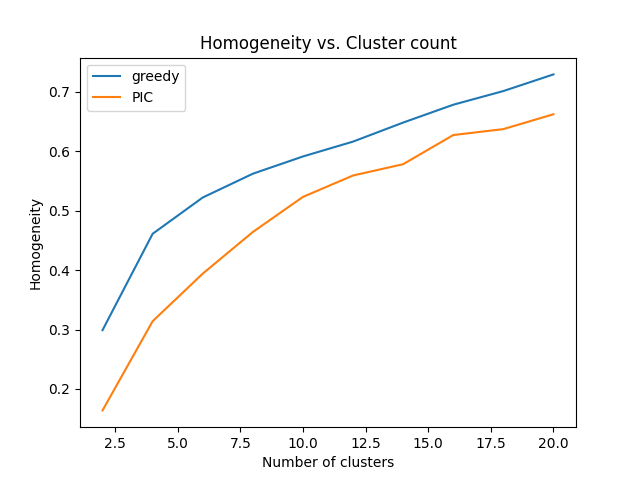
\includegraphics[width=0.45\textwidth]{assets/results/dbpediaProfiles/homogenity_comparison.png}
    \caption{Homogeneity vs Number of clusters for dbpediaProfiles data set}
    \label{fig:homogenity_dbpediaProfiles}
\end{figure}

\begin{figure}[H]
    \centering
    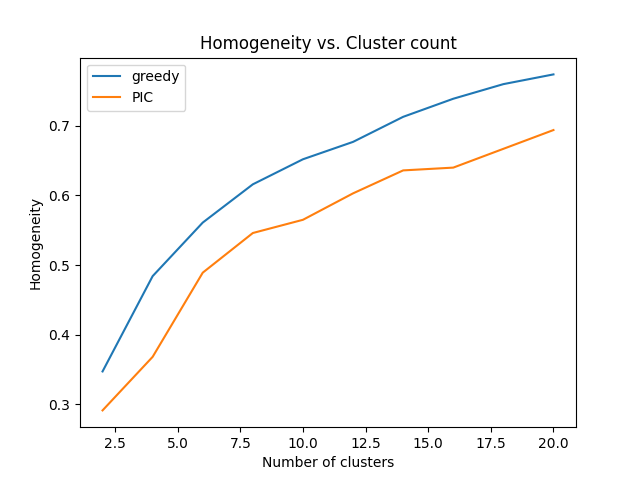
\includegraphics[width=0.45\textwidth]{assets/results/dunkin_stores/homogenity_comparison.png}
    \caption{Homogeneity vs Number of clusters for Dunkin stores data set}
    \label{fig:homogenity_dunkin_stores}
\end{figure}

\begin{figure}[H]
    \centering
    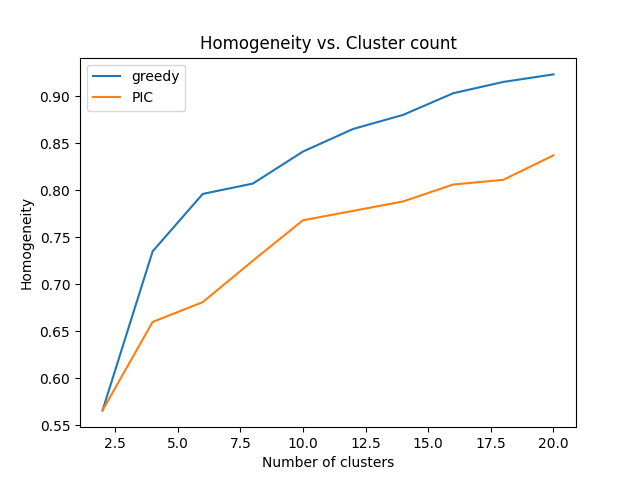
\includegraphics[width=0.45\textwidth]{assets/results/syntheticFincances/homogenity_comparison.png}
    \caption{Homogeneity vs Number of clusters for synthetic Finance data set}
    \label{fig:homogenity_syntheticFinance}
\end{figure}

\begin{figure}[H]
    \centering
    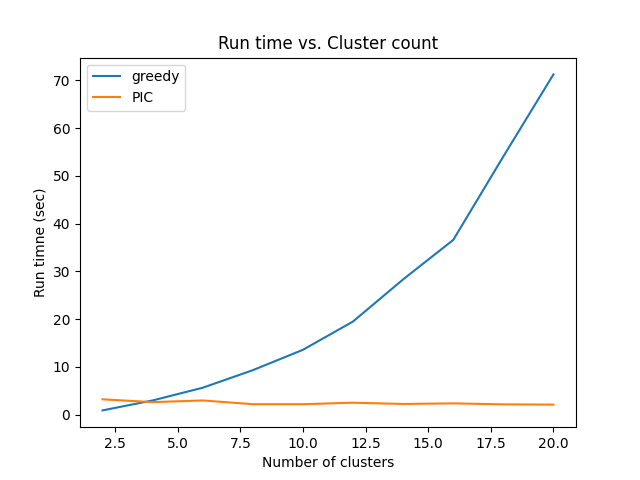
\includegraphics[width=0.45\textwidth]{assets/results/dbpediaProfiles/run_time_comparison.png}
    \caption{Run time vs Number of clusters for dbpediaProfiles data set}
    \label{fig:runtime_dbpediaProfiles}
\end{figure}

\begin{figure}[H]
    \centering
    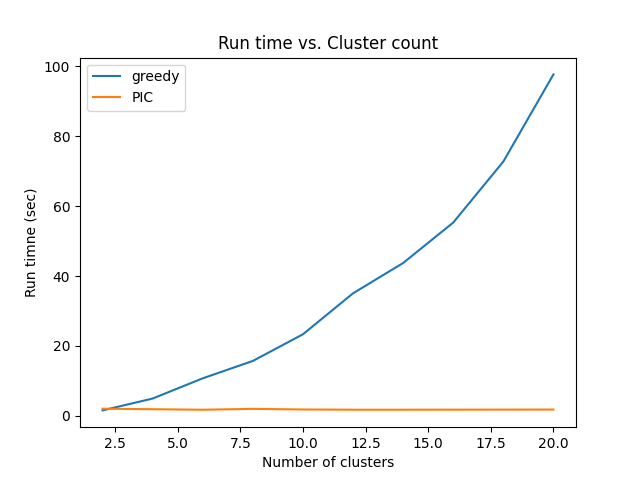
\includegraphics[width=0.45\textwidth]{assets/results/dunkin_stores/run_time_comparison.png}
    \caption{Run time vs Number of clusters for Dunkin stores data set}
    \label{fig:runtime_dunkin_stores}
\end{figure}

\begin{figure}[H]
    \centering
    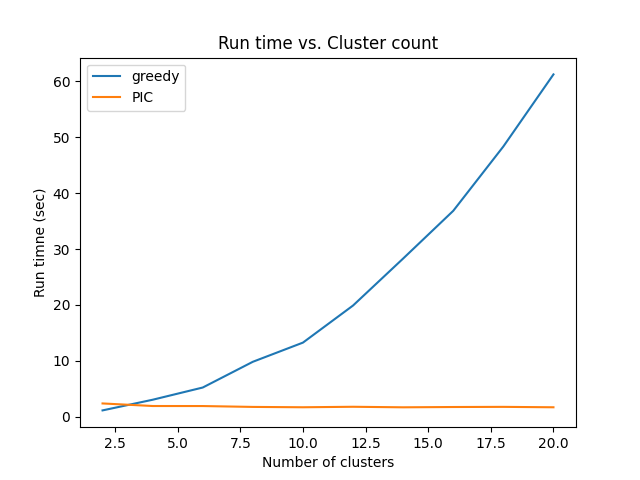
\includegraphics[width=0.45\textwidth]{assets/results/syntheticFincances/run_time_comparison.png}
    \caption{Run time vs Number of clusters for synthetic Finance stores data set}
    \label{fig:runtime_syntheticFinance}
\end{figure}

\clearpage

\begin{figure}
    \centering
    \resizebox{0.95\textwidth}{!}{\begin{tabular}[c]{cc}
    \begin{subfigure}[c]{0.45\textwidth}
         \centering
         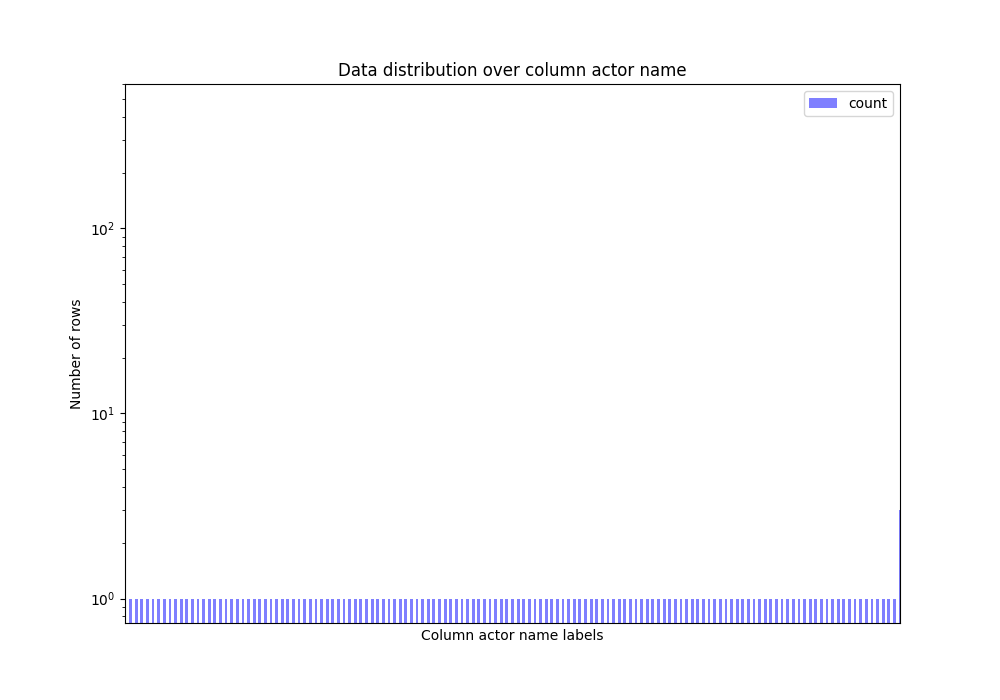
\includegraphics[width=\textwidth]{assets/results/dbpediaProfiles/distribution/actor name.png}
         \caption{Actor name}
         \label{}
     \end{subfigure} &
     \begin{subfigure}[c]{0.45\textwidth}
         \centering
         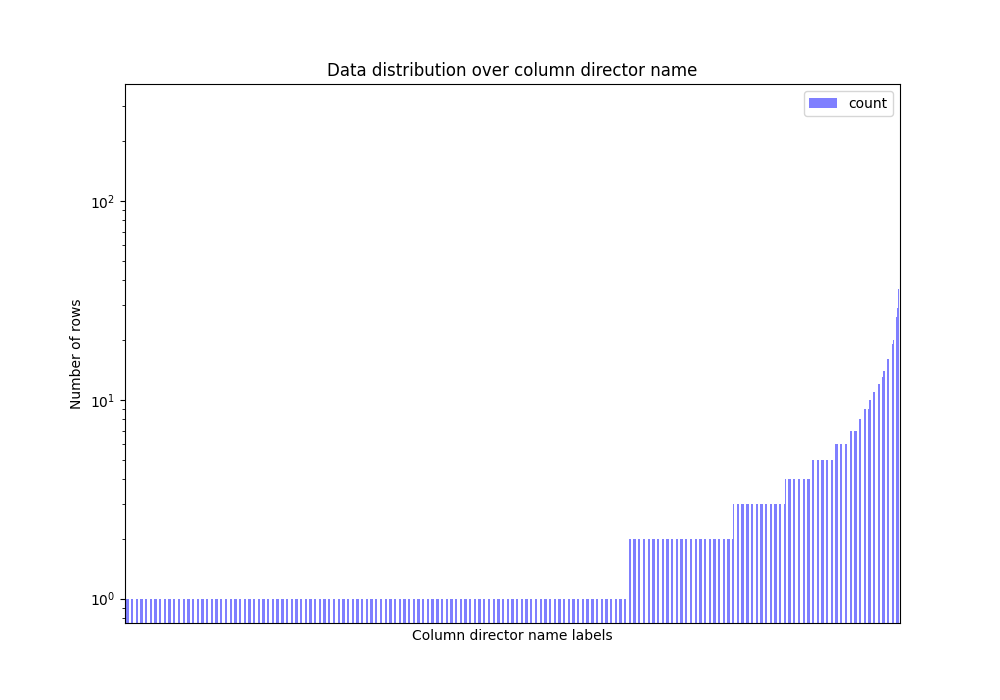
\includegraphics[width=\textwidth]{assets/results/dbpediaProfiles/distribution/director name.png}
         \caption{Director name}
         \label{}
     \end{subfigure} \\
     
     \begin{subfigure}[c]{0.45\textwidth}
         \centering
         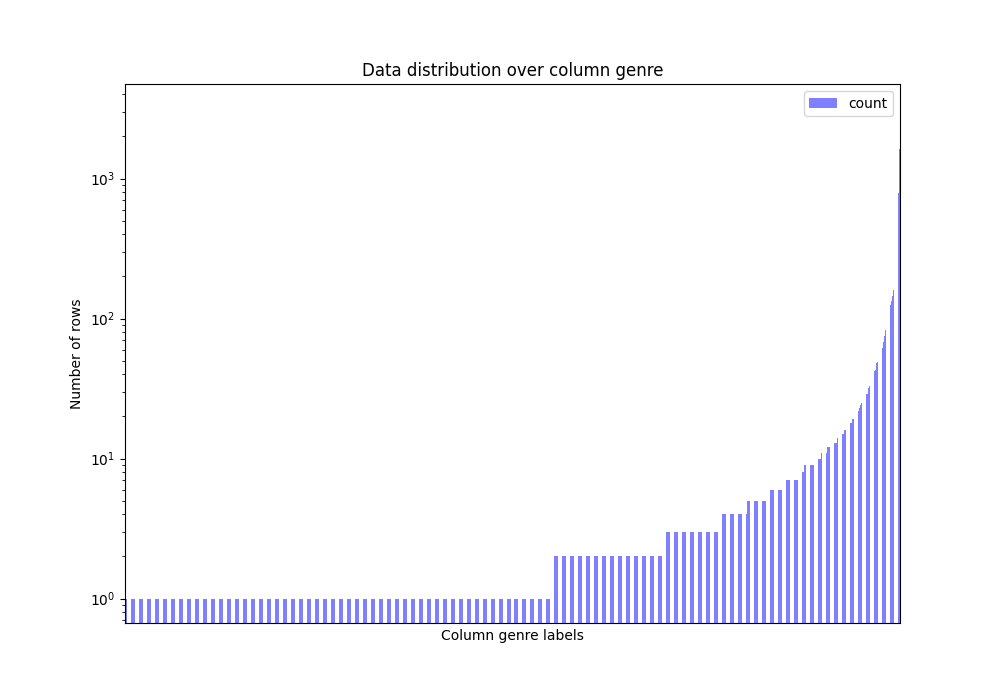
\includegraphics[width=\textwidth]{assets/results/dbpediaProfiles/distribution/genre.png}
         \caption{Genre}
         \label{}
     \end{subfigure} &
     \begin{subfigure}[c]{0.45\textwidth}
         \centering
         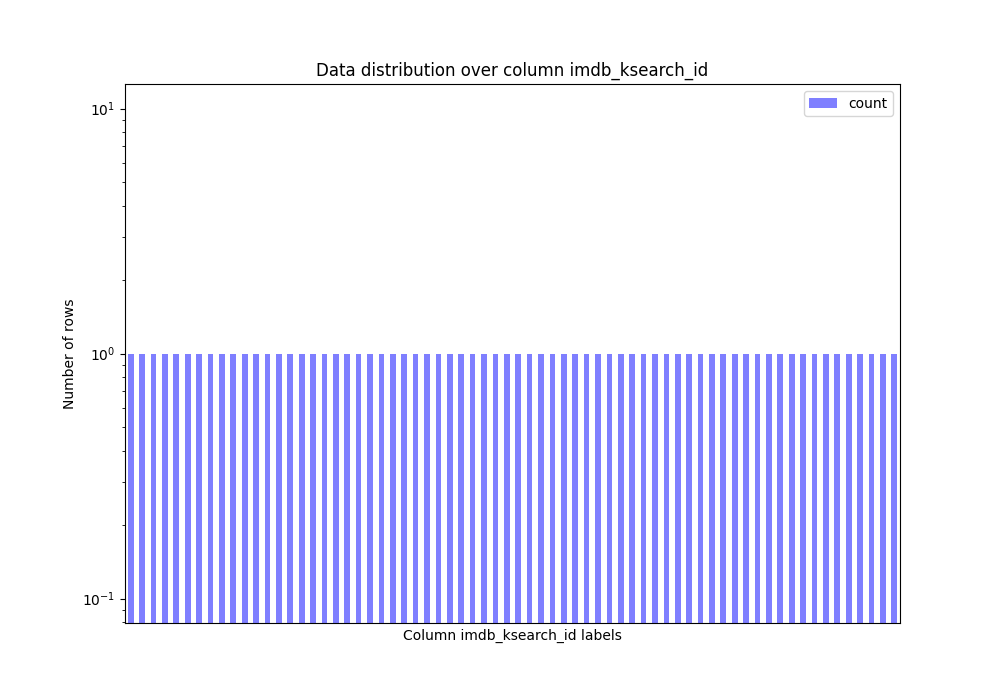
\includegraphics[width=\textwidth]{assets/results/dbpediaProfiles/distribution/imdb_ksearch_id.png}
         \caption{Imdb ksearch id}
         \label{}
     \end{subfigure} \\
     \begin{subfigure}[c]{0.45\textwidth}
         \centering
         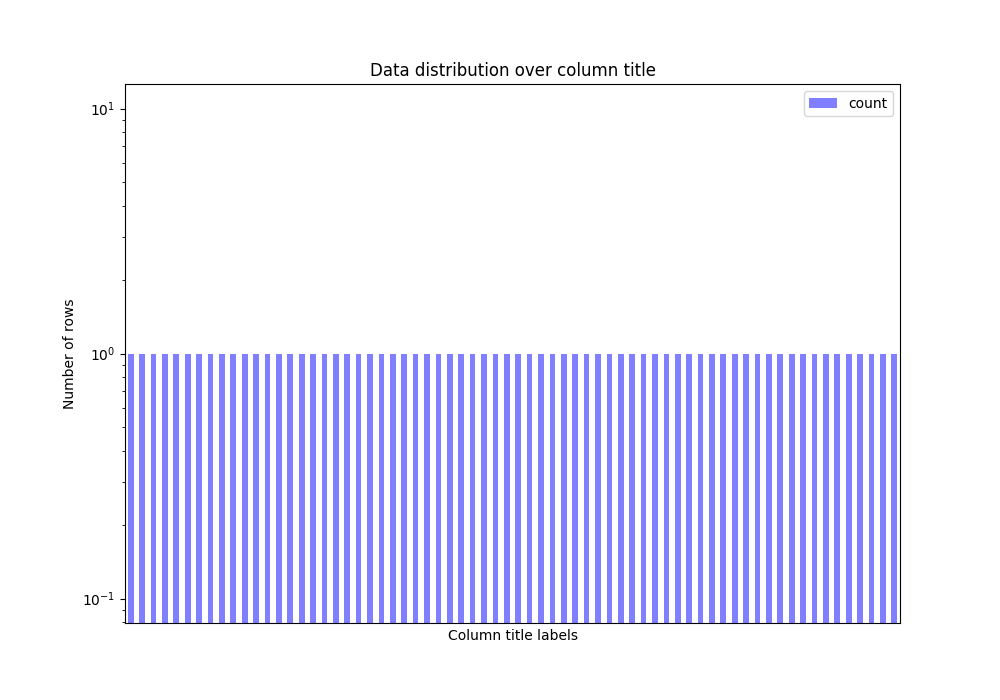
\includegraphics[width=\textwidth]{assets/results/dbpediaProfiles/distribution/title.png}
         \caption{Title}
         \label{}
     \end{subfigure} &
     \begin{subfigure}[c]{0.45\textwidth}
         \centering
         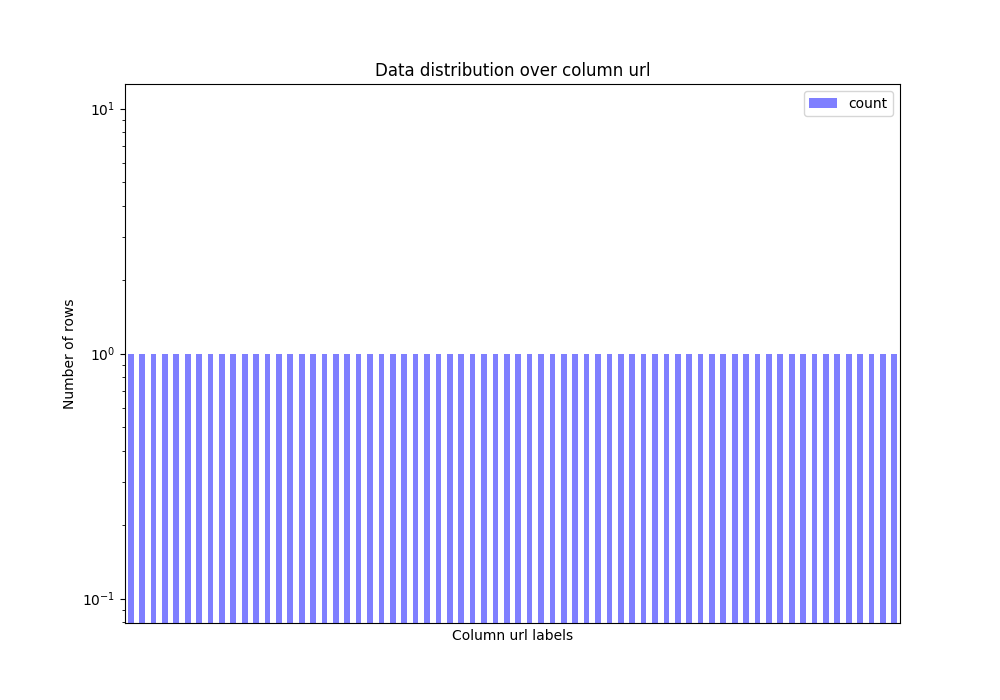
\includegraphics[width=\textwidth]{assets/results/dbpediaProfiles/distribution/url.png}
         \caption{Url}
         \label{}
     \end{subfigure} \\
     \multicolumn{2}{c}{\begin{subfigure}[c]{0.45\textwidth}
         \centering
         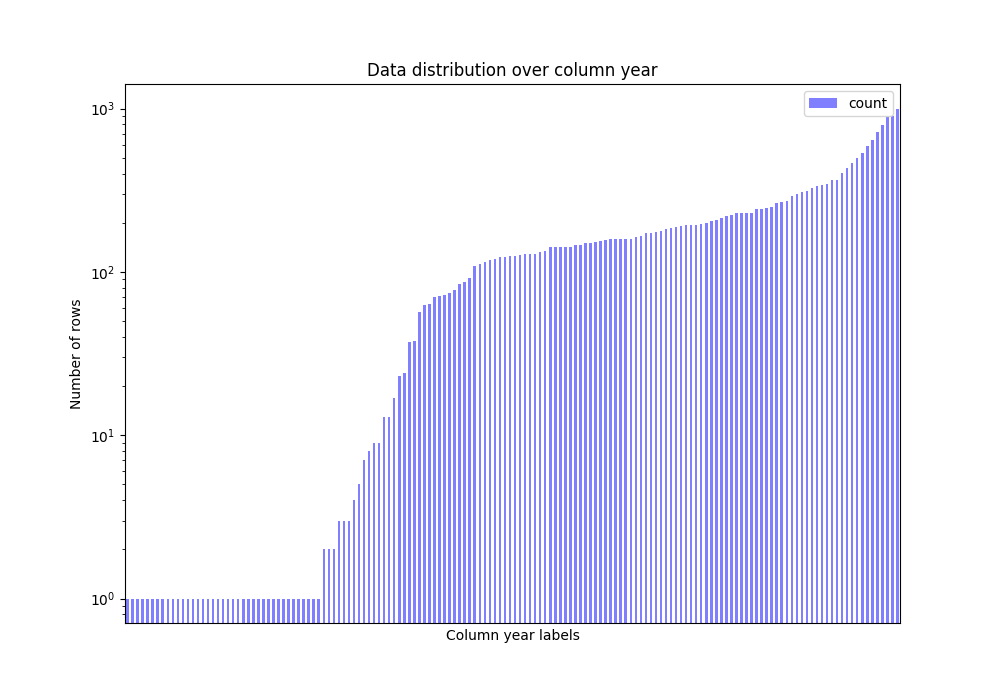
\includegraphics[width=\textwidth]{assets/results/dbpediaProfiles/distribution/year.png}
         \caption{Year}
         \label{}
     \end{subfigure}}
     \end{tabular}
     }
    \caption{Distribution analysis for dbpediaProfiles data set}
    \label{fig:dbpediaProfiles_distribution_analysis}
\end{figure}

\clearpage

\begin{figure}
    \centering
    \resizebox{0.7\textwidth}{!}{\begin{tabular}[c]{cc}
    \begin{subfigure}[c]{0.45\textwidth}
         \centering
         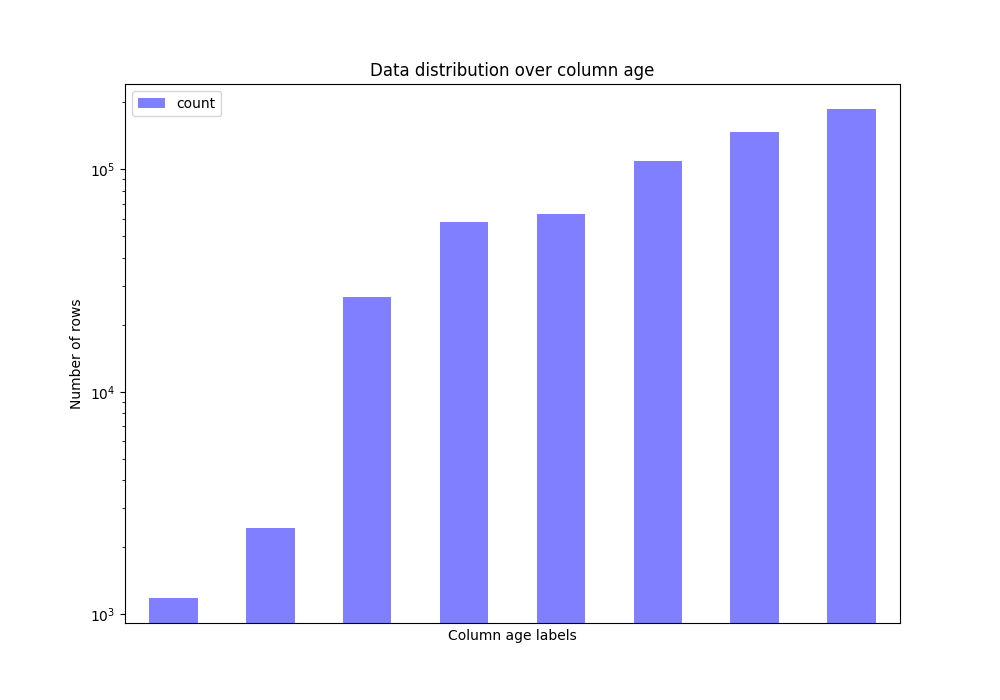
\includegraphics[width=\textwidth]{assets/results/syntheticFincances/distribution/age.png}
         \caption{Age}
         \label{}
     \end{subfigure} &
     
     \begin{subfigure}[c]{0.45\textwidth}
         \centering
         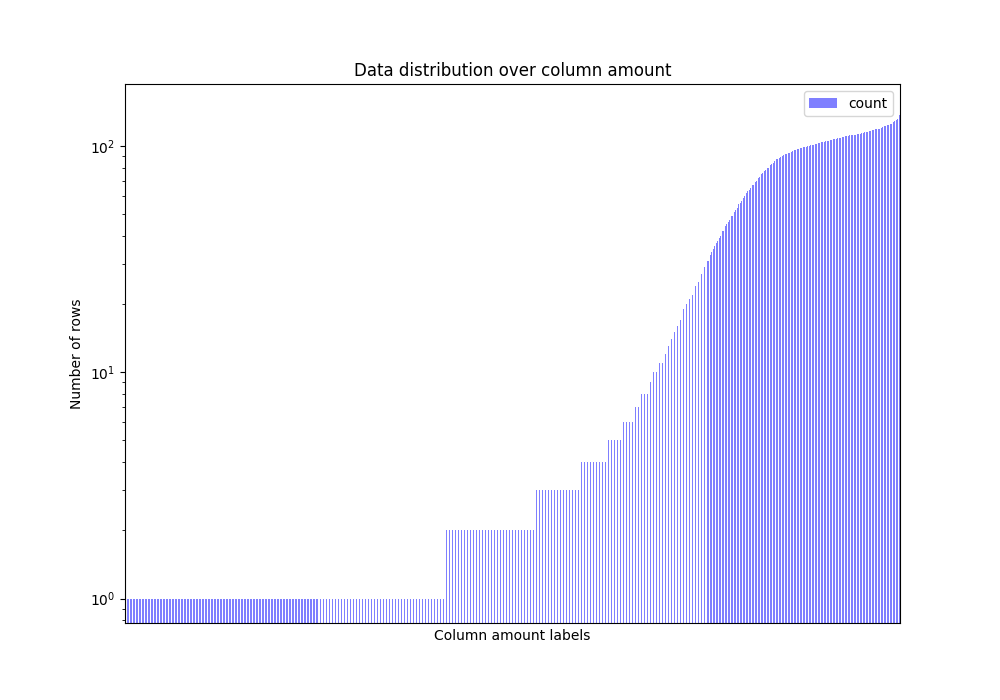
\includegraphics[width=\textwidth]{assets/results/syntheticFincances/distribution/amount.png}
         \caption{Amount}
         \label{}
     \end{subfigure} \\
     
     \begin{subfigure}[c]{0.45\textwidth}
         \centering
         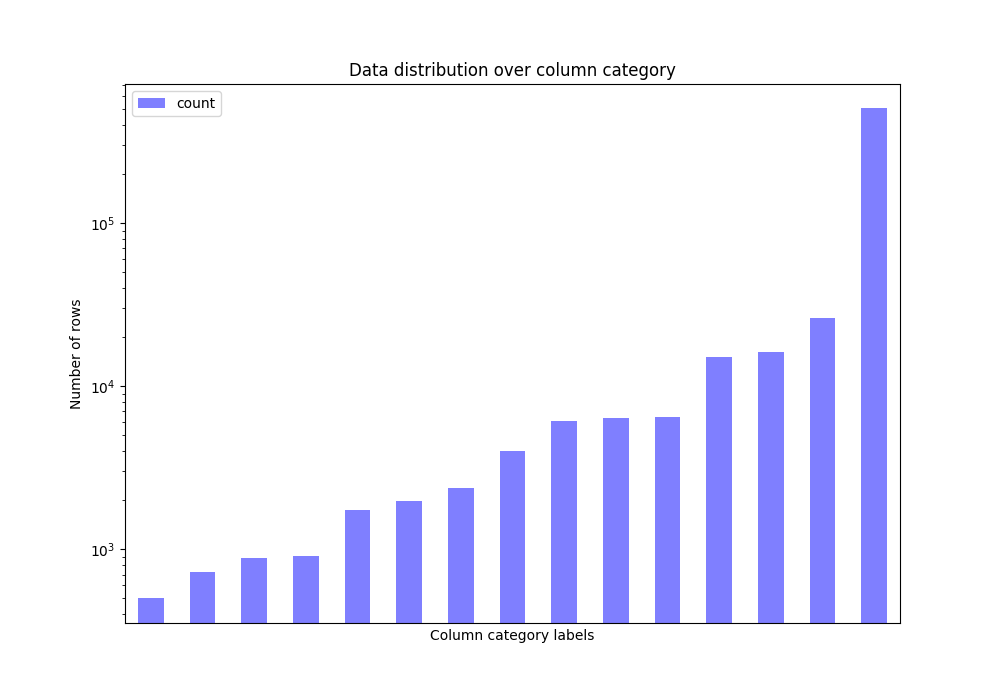
\includegraphics[width=\textwidth]{assets/results/syntheticFincances/distribution/category.png}
         \caption{Category}
         \label{}
     \end{subfigure} &
     
     \begin{subfigure}[c]{0.45\textwidth}
         \centering
         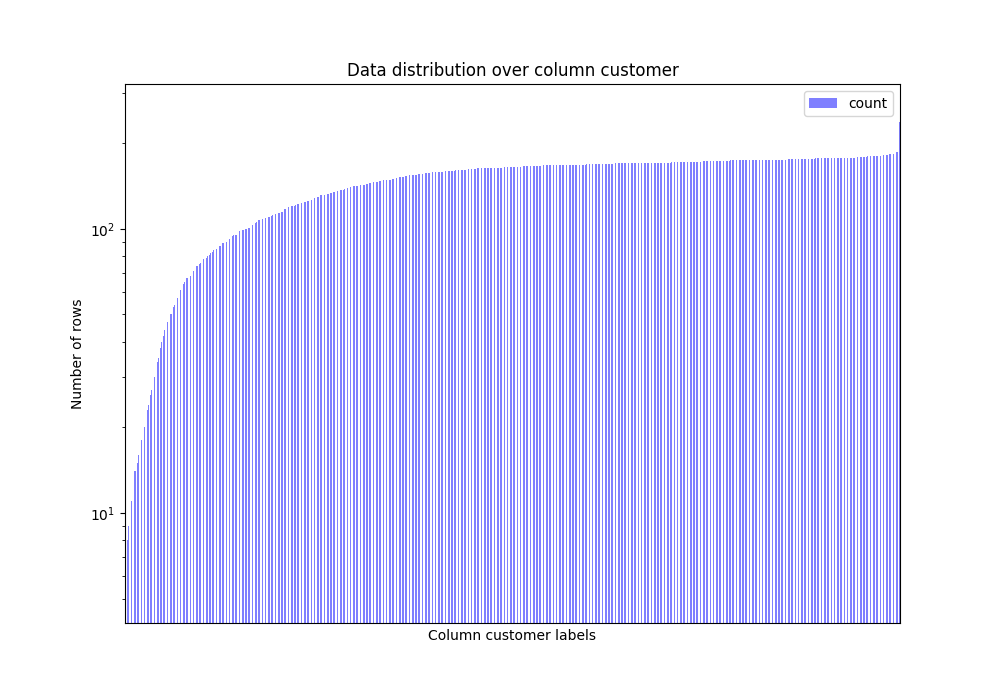
\includegraphics[width=\textwidth]{assets/results/syntheticFincances/distribution/customer.png}
         \caption{Customer}
         \label{}
     \end{subfigure} \\
     
     \begin{subfigure}[c]{0.45\textwidth}
         \centering
         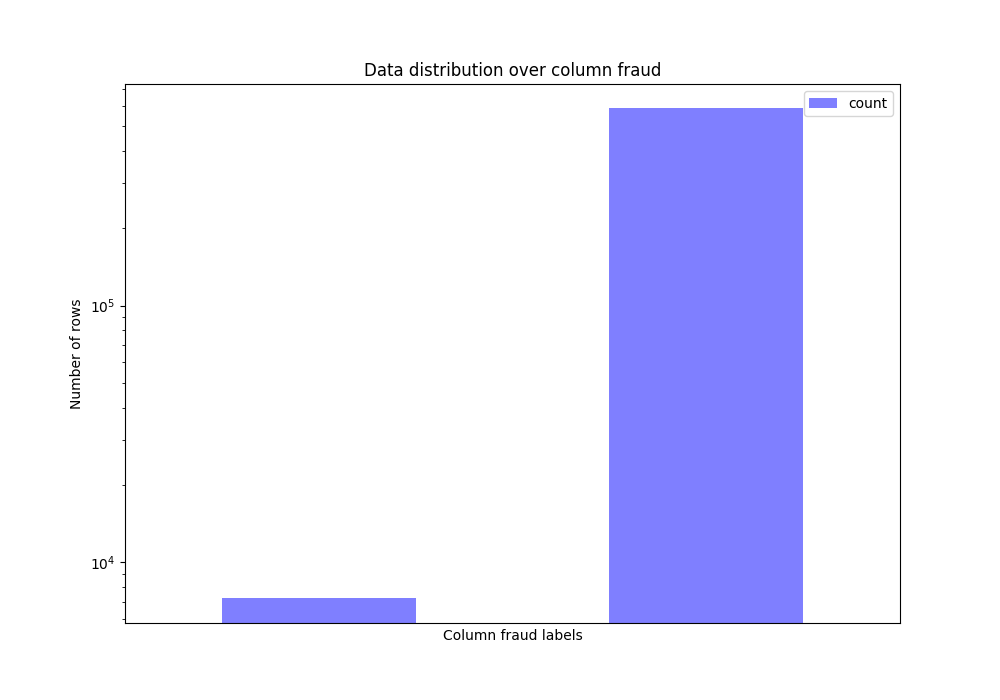
\includegraphics[width=\textwidth]{assets/results/syntheticFincances/distribution/fraud.png}
         \caption{Fraud}
         \label{}
     \end{subfigure} &
     
     \begin{subfigure}[c]{0.45\textwidth}
         \centering
         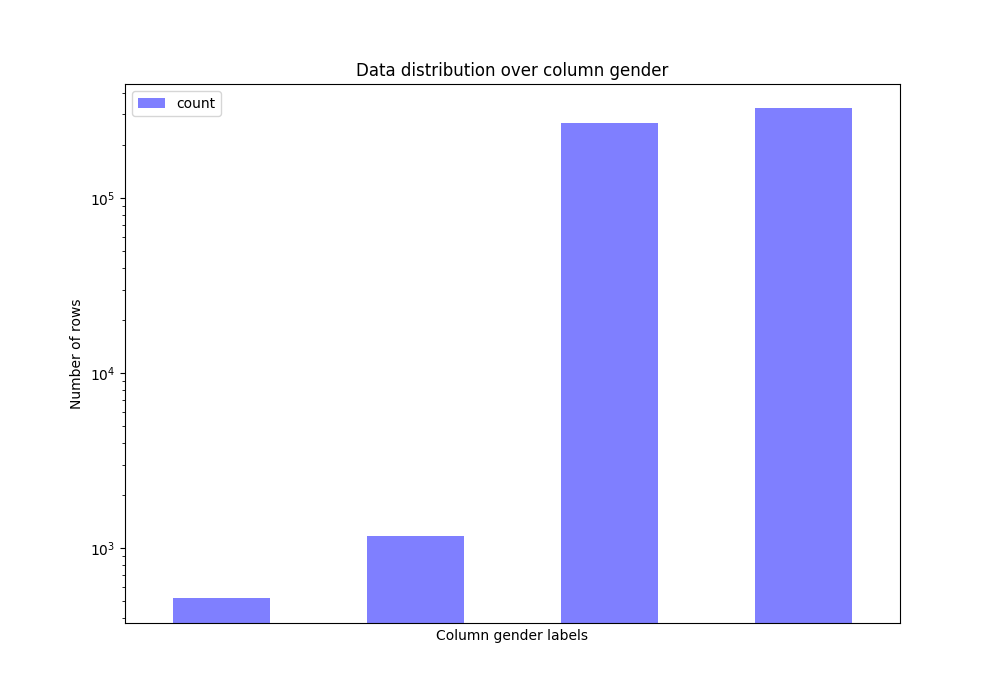
\includegraphics[width=\textwidth]{assets/results/syntheticFincances/distribution/gender.png}
         \caption{Gender}
         \label{}
     \end{subfigure}  \\
     
     \begin{subfigure}[c]{0.45\textwidth}
         \centering
         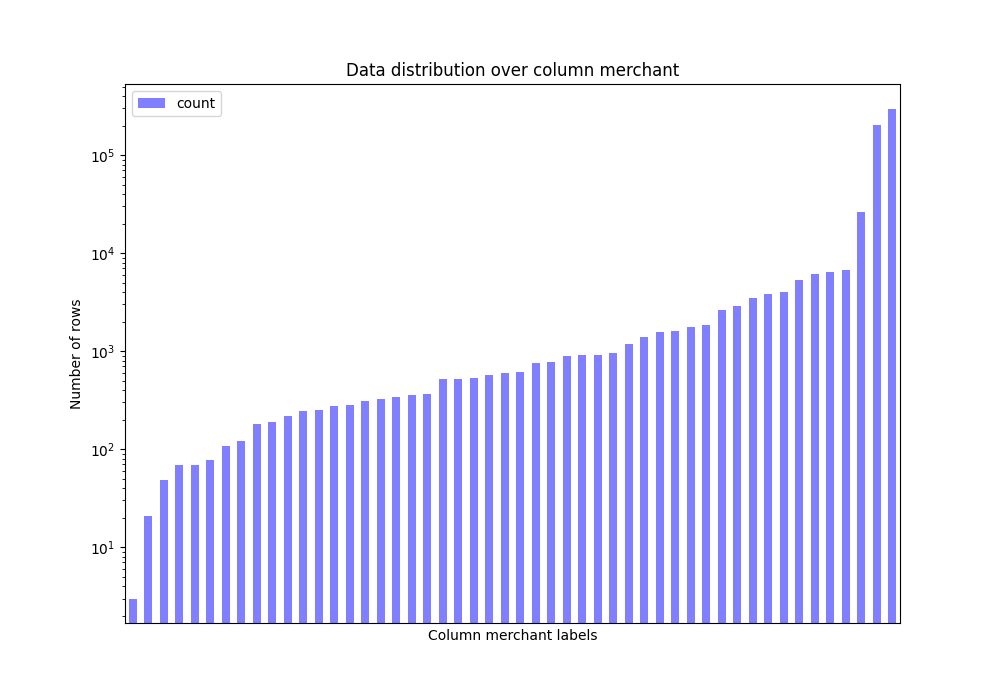
\includegraphics[width=\textwidth]{assets/results/syntheticFincances/distribution/merchant.png}
         \caption{Merchant}
         \label{}
     \end{subfigure} &
     
     \begin{subfigure}[c]{0.45\textwidth}
         \centering
         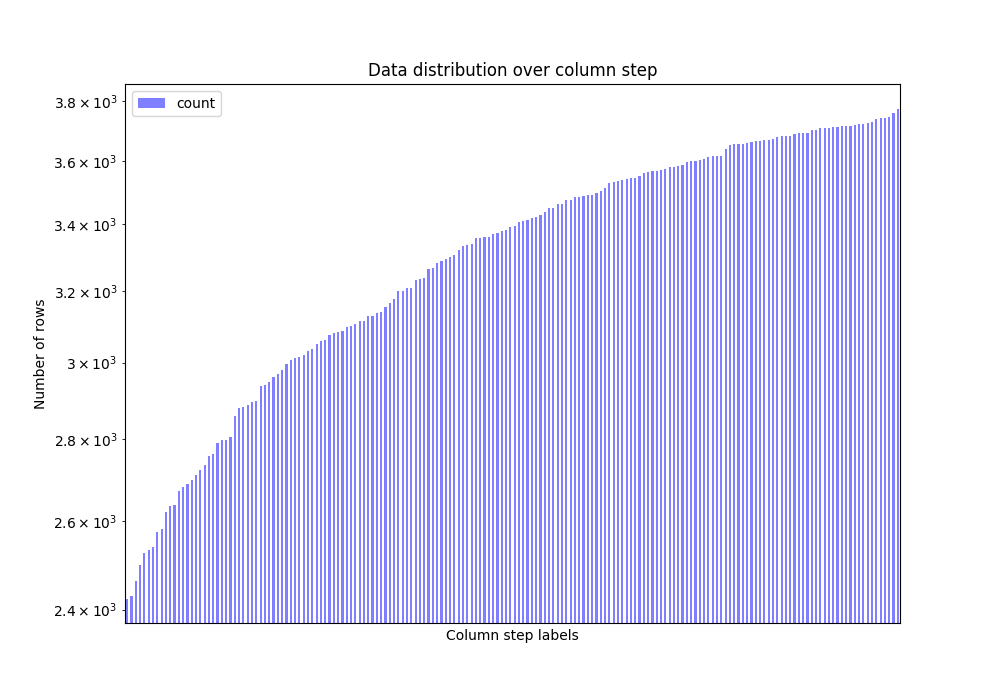
\includegraphics[width=\textwidth]{assets/results/syntheticFincances/distribution/step.png}
         \caption{Step}
         \label{}
     \end{subfigure} \\
     
     \begin{subfigure}[c]{0.45\textwidth}
         \centering
         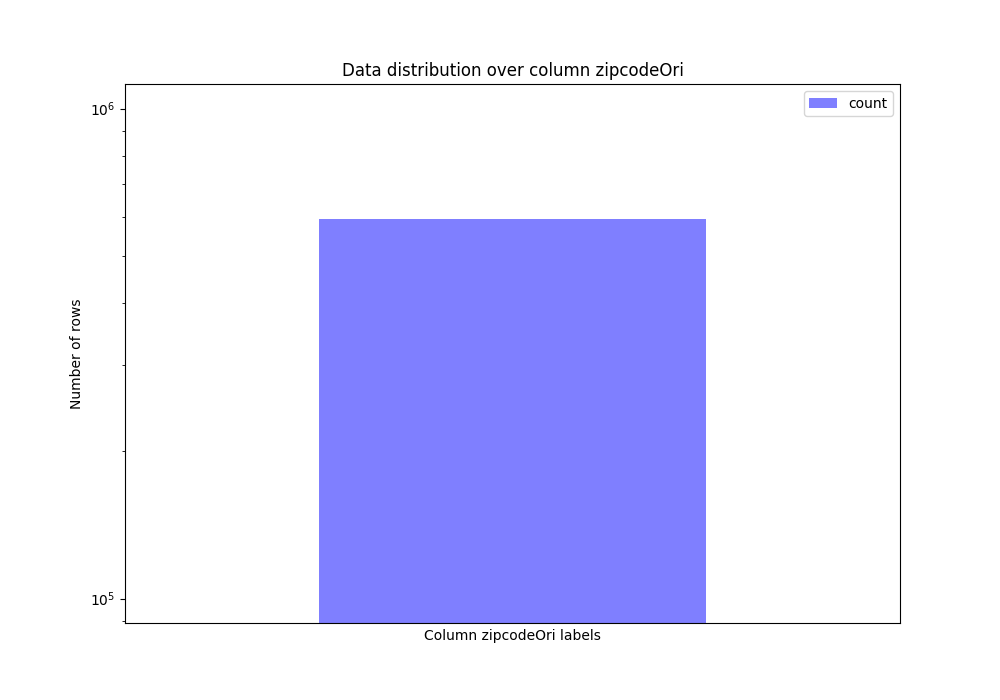
\includegraphics[width=\textwidth]{assets/results/syntheticFincances/distribution/zipcodeOri.png}
         \caption{zipcodeOri}
         \label{}
     \end{subfigure} &
     
     \begin{subfigure}[c]{0.45\textwidth}
         \centering
         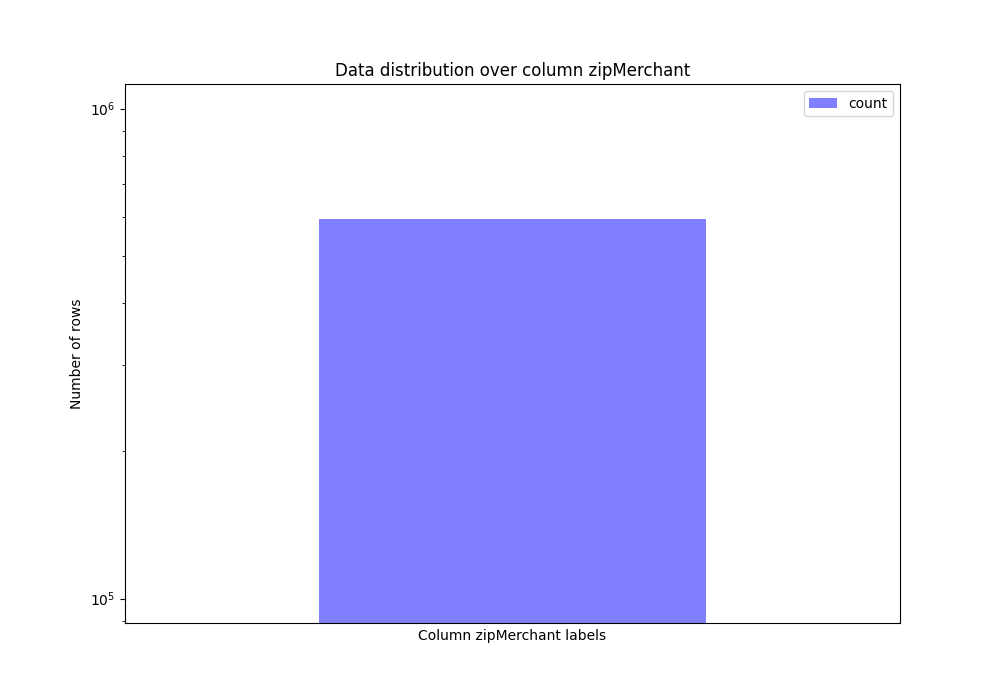
\includegraphics[width=\textwidth]{assets/results/syntheticFincances/distribution/zipMerchant.png}
         \caption{zipMerchant}
         \label{}
     \end{subfigure} 
     \end{tabular} 
     }
    \caption{Distribution analysis for synthetic Finance}
    \label{fig:synthetic_finance_distribution_analysis}
\end{figure}

\end{document}
